\beginsong{An den sechs vergang'nen Tagen}[wuw={Alf Zschiesche}, bo={26}, pfii={28}, pfiii={55}]

\markboth{\songtitle}{\songtitle}

\beginverse
\endverse

\centering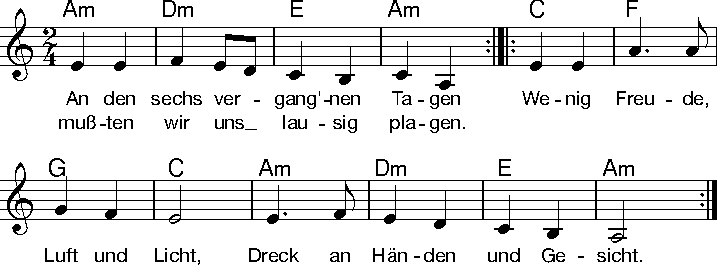
\includegraphics[width=1\textwidth]{Noten/Lied102.pdf}

\beginverse
\[Am]Heute \[Dm]hat die \[E]Welt uns \[Am]wieder, Klampfen\[Dm]spiel und \[E]hundert \[Am]Lieder,
\lrep \[C]wandern \[F]durch die \[G]Wälder \[C]mit \[Am]zu dem \[Dm]Sieben\[E]meilen\[Am]schritt. \rrep
\endverse

\beginverse
^Und so ^geht es ^immer ^munter Berge ^rauf und ^wieder ^runter,
\lrep ^alle ^uns're ^Müdig^keit ^steckt zu^haus im ^Arbeits^kleid. \rrep
\endverse

\beginverse 
^Sieben ^Tage ^hat die ^Woche, sechse ^sind wir ^rumge^krochen,
\lrep ^doch am ^siebten ^lebt sich's ^flott, ^also ^will's der ^liebe ^Gott. \rrep
\endverse

\endsong

%\beginscripture
%\endscripture

\begin{intersong}

\end{intersong}